\documentclass[10pt]{beamer}
\usetheme{metropolis}
\usepackage{booktabs}
\usepackage{tabularx}
\usepackage{calc}
\usepackage{tikz}

% Setup for faculty images
\newlength{\imageheight}
\setlength{\imageheight}{3.5cm}

% Define CSUF brand colors
\definecolor{titanblue}{HTML}{00244E}
\definecolor{mediumblue}{HTML}{0F3F8C}
\definecolor{skyblue}{HTML}{EBFBFF}
\definecolor{titanorange}{HTML}{FF7900}
\definecolor{titangray}{HTML}{F5F5F5}
\definecolor{titantext}{HTML}{222222}

% Additional vibrant colors for theories
\definecolor{streamblue}{HTML}{2563EB}
\definecolor{streamgreen}{HTML}{059669}
\definecolor{streampurple}{HTML}{7C3AED}
\definecolor{coalitionred}{HTML}{DC2626}
\definecolor{coalitionblue}{HTML}{2563EB}
\definecolor{punctuationorange}{HTML}{EA580C}
\definecolor{equilibriumgreen}{HTML}{059669}

% Customize metropolis theme colors
\setbeamercolor{normal text}{fg=titantext, bg=white}
\setbeamercolor{alerted text}{fg=titanorange}
\setbeamercolor{example text}{fg=mediumblue}

% Title page colors
\setbeamercolor{title}{fg=titanblue, bg=white}
\setbeamercolor{subtitle}{fg=mediumblue, bg=white}
\setbeamercolor{institute}{fg=titanorange, bg=white}
\setbeamercolor{date}{fg=titanblue, bg=white}

% Frame title colors
\setbeamercolor{frametitle}{fg=white, bg=titanblue}
\setbeamercolor{framesubtitle}{fg=mediumblue, bg=white}

% Block environment colors
\setbeamercolor{block title}{fg=white, bg=titanblue}
\setbeamercolor{block body}{fg=titantext, bg=skyblue!10}

% Different block types
\setbeamercolor{block title example}{fg=white, bg=equilibriumgreen}
\setbeamercolor{block body example}{fg=titantext, bg=equilibriumgreen!10}

\setbeamercolor{block title alerted}{fg=white, bg=punctuationorange}
\setbeamercolor{block body alerted}{fg=titantext, bg=punctuationorange!10}

% Item colors
\setbeamercolor{itemize item}{fg=titanorange}
\setbeamercolor{itemize subitem}{fg=mediumblue}
\setbeamercolor{itemize subsubitem}{fg=titanblue}

% Footer and header colors
\setbeamercolor{footer}{fg=titantext}
\setbeamercolor{header}{fg=titanblue}

% Customize fonts
\setbeamerfont{title}{size=\Large, series=\bfseries}
\setbeamerfont{frametitle}{size=\large, series=\bfseries}

% Custom section slide template
\defbeamertemplate{background}{section}{%
  \begin{tikzpicture}[remember picture,overlay]
    \fill[titanorange,opacity=0.9] (current page.south west) rectangle (current page.north east);
  \end{tikzpicture}
}

% Simple title page template
\defbeamertemplate*{title page}{customized}[1][]
{
  \vspace{1cm}
  {\usebeamerfont{title}\usebeamercolor[fg]{title}\inserttitle\par}
  \vspace{0.5cm}
  {\usebeamerfont{subtitle}\usebeamercolor[fg]{subtitle}\insertsubtitle\par}
  \vspace{0.5cm}
  {\usebeamerfont{date}\usebeamercolor[fg]{date}\insertdate\par}
  \vfill
  {\usebeamercolor[fg]{institute}\insertinstitute\par}
  \vfill
  {\small David P. Adams, Ph.D.\par}
}

% Apply the custom title page template
\setbeamertemplate{title page}[customized]

% Define a beamer color for the headline background
\setbeamercolor{headline}{bg=titanblue}

% Add progress bar to the headline
\makeatletter
\setbeamertemplate{headline}{%
  \begin{beamercolorbox}[wd=\paperwidth,ht=0.4cm,dp=0cm]{headline}%
    \begin{tikzpicture}[overlay, remember picture]
      % Draw a titanorange rectangle whose width is the fraction:
      % \insertframenumber / \inserttotalframenumber of the paper width,
      % and height is 0.4cm.
      \fill[titanorange]
        (current page.south west) rectangle
        ($ (current page.south west) !\insertframenumber/\inserttotalframenumber! (current page.south east) + (0,0.4cm) $);
    \end{tikzpicture}%
  \end{beamercolorbox}%
}
\makeatother

\begin{document}

\title{Understanding Policy Change}
\subtitle{Introduction to Policy Process Theories\\POSC 315: Introduction to Public Policy\\Lecture 2-3}
\date{Summer 2025}
\institute{California State University, Fullerton}

\maketitle

% Introduction
\begin{frame}
\frametitle{What Is Policy Change?}

\begin{block}{}
  \centering
  Policy change refers to significant shifts in government action, law, or regulation over time.
\end{block}

\vspace{0.5cm}

\begin{itemize}
  \item Why do some policies stay the same for decades, while others change rapidly?
  \item What triggers major reforms or reversals?
  \item How do ideas, interests, and institutions interact to shape outcomes?
\end{itemize}

\pause
\vspace{0.5cm}

\begin{alertblock}{Today's Goal:}
  Introduce the main theories that help us answer these questions.
\end{alertblock}

\end{frame}

% Why Study Policy Process Theories
\begin{frame}
\frametitle{Why Study Policy Process Theories?}

\begin{block}{}
  \centering
  Theories help us:
\end{block}

\vspace{0.5cm}

\begin{columns}
  \begin{column}{0.48\textwidth}
    \begin{block}{1. Understand Change}
      \pause
      Make sense of how and why policies evolve over time
    \end{block}

    \vspace{0.3cm}

    \begin{block}{3. Predict Change}
      \pause
      Anticipate when conditions are ripe for policy shifts
    \end{block}
  \end{column}

  \begin{column}{0.48\textwidth}
    \begin{block}{2. Identify Key Factors}
      \pause
      Recognize the crucial elements that drive policy development
    \end{block}

    \vspace{0.3cm}

    \begin{block}{4. Analyze History}
      \pause
      Examine past policy successes and failures through theoretical lenses
    \end{block}
  \end{column}
\end{columns}

\end{frame}

% Major Theories Overview
\begin{frame}
\frametitle{Three Major Theoretical Frameworks}

\begin{columns}
  \begin{column}{0.32\textwidth}
    \begin{block}{\textcolor{streamblue}{Multiple Streams}}
      \pause
      \centering
      Policy windows open when problem, policy, and politics streams converge
    \end{block}
  \end{column}

  \begin{column}{0.32\textwidth}
    \begin{block}{\textcolor{coalitionred}{Advocacy Coalition}}
      \pause
      \centering
      Policy change through competing coalitions with shared belief systems
    \end{block}
  \end{column}

  \begin{column}{0.32\textwidth}
    \begin{block}{\textcolor{punctuationorange}{Punctuated Equilibrium}}
      \pause
      \centering
      Long periods of stability interrupted by sudden, dramatic shifts
    \end{block}
  \end{column}
\end{columns}

\pause
\vspace{1cm}
\centering
Each theory offers a different lens for examining policy change

\end{frame}

% Section: Multiple Streams
{
\setbeamertemplate{background}[section]
\begin{frame}[plain]
  \vspace{2cm}
  \begin{center}
    {\Huge\color{white}\textbf{Kingdon's Multiple Streams}}

    \vspace{0.5cm}
    {\Large\color{white}Framework}
  \end{center}
\end{frame}
}

% Multiple Streams Framework
\begin{frame}
\frametitle{Kingdon's Multiple Streams Framework}

\begin{block}{}
  \centering
  Policy windows open when three independent streams converge:
\end{block}

\vspace{0.5cm}

\begin{columns}
  \begin{column}{0.32\textwidth}
    \begin{block}{\textcolor{streamblue}{1. Problem Stream}}
      \pause
      Issues gaining attention

      \vspace{0.3cm}
      \small\emph{Example: Opioid crisis or rising homelessness}
    \end{block}
  \end{column}

  \begin{column}{0.32\textwidth}
    \begin{block}{\textcolor{streamgreen}{2. Policy Stream}}
      \pause
      Available solutions

      \vspace{0.3cm}
      \small\emph{Example: Harm reduction or housing-first policies}
    \end{block}
  \end{column}

  \begin{column}{0.32\textwidth}
    \begin{block}{\textcolor{streampurple}{3. Politics Stream}}
      \pause
      Political conditions

      \vspace{0.3cm}
      \small\emph{Example: Bipartisan support or public demand}
    \end{block}
  \end{column}
\end{columns}

\end{frame}

% Multiple Streams Visualization
\begin{frame}
\frametitle{Multiple Streams: When Streams Converge}

\begin{columns}
  \begin{column}{0.55\textwidth}
    \begin{center}
      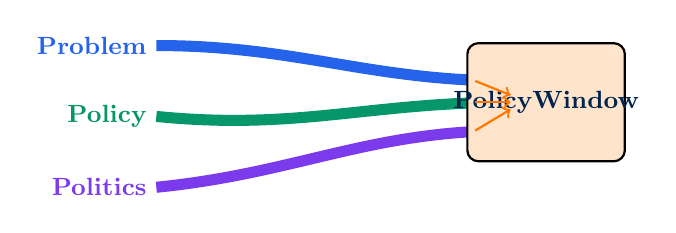
\begin{tikzpicture}[scale=0.9]
        % Draw the three streams
        \draw[thick, streamblue, line width=4pt] (0,3) .. controls (2,3) and (3,2.5) .. (5,2.5);
        \draw[thick, streamgreen, line width=4pt] (0,2) .. controls (2,1.8) and (3,2.2) .. (5,2.2);
        \draw[thick, streampurple, line width=4pt] (0,1) .. controls (2,1.2) and (3,1.8) .. (5,1.8);

        % Policy window
        \node[draw, thick, fill=titanorange!20, minimum width=2cm, minimum height=1.5cm, rounded corners] at (5.5,2.2) {};
        \node[text=titanblue, font=\small\bfseries] at (5.5,2.2) {Policy\\Window};

        % Stream labels
        \node[left, text=streamblue, font=\small\bfseries] at (0,3) {Problem};
        \node[left, text=streamgreen, font=\small\bfseries] at (0,2) {Policy};
        \node[left, text=streampurple, font=\small\bfseries] at (0,1) {Politics};

        % Convergence arrows
        \draw[->, thick, titanorange] (4.5,2.5) -- (5,2.3);
        \draw[->, thick, titanorange] (4.5,2.2) -- (5,2.2);
        \draw[->, thick, titanorange] (4.5,1.8) -- (5,2.1);
      \end{tikzpicture}
    \end{center}
  \end{column}

  \begin{column}{0.45\textwidth}
    \begin{block}{Key Actors}
      \pause
      \begin{itemize}
        \item \textbf{Policy Entrepreneurs}: Individuals who promote solutions and connect streams
        \item \textbf{Policy Windows}: Brief opportunities for policy change  
        \item \textbf{Coupling}: The process of linking problems to solutions in the right political moment
      \end{itemize}
    \end{block}
  \end{column}
\end{columns}

\pause
\vspace{0.5cm}

\begin{alertblock}{Real-World Example:}
  The Clean Air Act amendments of 1990, where environmental concerns, available policy solutions, and bipartisan political support converged at the right moment.
\end{alertblock}

\end{frame}

% Section: Advocacy Coalition
{
\setbeamertemplate{background}[section]
\begin{frame}[plain]
  \vspace{2cm}
  \begin{center}
    {\Huge\color{white}\textbf{Advocacy Coalition}}

    \vspace{0.5cm}
    {\Large\color{white}Framework}
  \end{center}
\end{frame}
}

% Advocacy Coalition Framework
\begin{frame}
\frametitle{Advocacy Coalition Framework}

\begin{block}{}
  \centering
  Policy change occurs through competing coalitions organized around shared beliefs
\end{block}

\vspace{0.5cm}

\begin{columns}
  \begin{column}{0.32\textwidth}
    \begin{block}{1. Shared Beliefs}
      \pause
      Groups form around common values and policy goals
    \end{block}
  \end{column}

  \begin{column}{0.32\textwidth}
    \begin{block}{2. Competition}
      \pause
      Coalitions compete to influence policy decisions
    \end{block}
  \end{column}

  \begin{column}{0.32\textwidth}
    \begin{block}{3. Adaptation}
      \pause
      Coalitions learn and adjust strategies over time
    \end{block}
  \end{column}
\end{columns}

\end{frame}

% Advocacy Coalition Visualization
\begin{frame}
\frametitle{Advocacy Coalition Framework: Structure}

\begin{columns}
  \begin{column}{0.55\textwidth}
    \begin{center}
      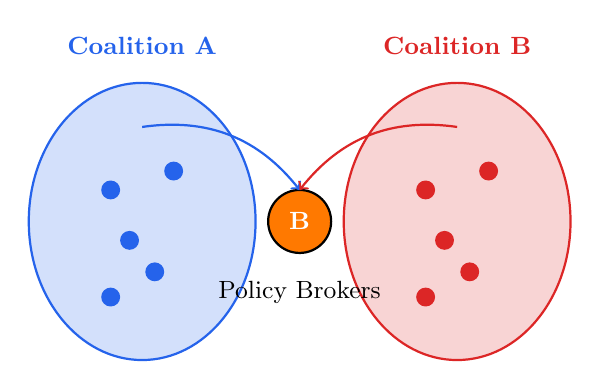
\begin{tikzpicture}[scale=0.8]
        % Coalition A
        \draw[thick, coalitionblue, fill=coalitionblue!20] (-1,0) ellipse (1.8cm and 2.2cm);
        \node[above, text=coalitionblue, font=\small\bfseries] at (-1,2.5) {Coalition A};

        % Coalition B
        \draw[thick, coalitionred, fill=coalitionred!20] (4,0) ellipse (1.8cm and 2.2cm);
        \node[above, text=coalitionred, font=\small\bfseries] at (4,2.5) {Coalition B};

        % Coalition A members
        \foreach \x/\y in {-1.5/0.5, -0.5/0.8, -1.2/-0.3, -0.8/-0.8, -1.5/-1.2} {
          \fill[coalitionblue] (\x,\y) circle (0.15);
        }

        % Coalition B members  
        \foreach \x/\y in {3.5/0.5, 4.5/0.8, 3.8/-0.3, 4.2/-0.8, 3.5/-1.2} {
          \fill[coalitionred] (\x,\y) circle (0.15);
        }

        % Policy brokers in middle
        \node[draw, thick, circle, fill=titanorange, text=white, minimum size=0.8cm] at (1.5,0) {\small\textbf{B}};
        \node[below, font=\small] at (1.5,-0.8) {Policy Brokers};

        % Competition arrows
        \draw[->, thick, coalitionblue, bend left=30] (-1,1.5) to (1.5,0.5);
        \draw[->, thick, coalitionred, bend right=30] (4,1.5) to (1.5,0.5);
      \end{tikzpicture}
    \end{center}
  \end{column}

  \begin{column}{0.45\textwidth}
    \begin{block}{Key Concepts}
      \pause
      \begin{itemize}
        \item \textbf{Belief Systems}: Core values that unite coalition members
        \item \textbf{Policy Subsystems}: Specific policy areas where coalitions compete
        \item \textbf{Policy Learning}: How coalitions adapt their strategies based on experience
      \end{itemize}
    \end{block}
  \end{column}
\end{columns}

\pause
\vspace{0.5cm}

\begin{alertblock}{Real-World Example:}
  The long-term debate between environmental advocates and the fossil fuel industry over climate policy, with each coalition learning and adapting strategies over decades.
\end{alertblock}

\end{frame}

% Section: Punctuated Equilibrium
{
\setbeamertemplate{background}[section]
\begin{frame}[plain]
  \vspace{2cm}
  \begin{center}
    {\Huge\color{white}\textbf{Punctuated Equilibrium}}

    \vspace{0.5cm}
    {\Large\color{white}Theory}
  \end{center}
\end{frame}
}

% Punctuated Equilibrium Theory
\begin{frame}
\frametitle{Punctuated Equilibrium Theory}

\begin{block}{}
  \centering
  Policy changes through long periods of stability interrupted by sudden, dramatic shifts
\end{block}

\vspace{0.5cm}

\begin{columns}
  \begin{column}{0.32\textwidth}
    \begin{block}{\textcolor{equilibriumgreen}{1. Stability}}
      \pause
      Long periods of incremental change or no change
    \end{block}
  \end{column}

  \begin{column}{0.32\textwidth}
    \begin{block}{\textcolor{punctuationorange}{2. Punctuation}}
      \pause
      Sudden, dramatic policy shifts
    \end{block}
  \end{column}

  \begin{column}{0.32\textwidth}
    \begin{block}{\textcolor{equilibriumgreen}{3. New Equilibrium}}
      \pause
      Return to stability at a new policy position
    \end{block}
  \end{column}
\end{columns}

\end{frame}

% Punctuated Equilibrium Visualization
\begin{frame}
\frametitle{Punctuated Equilibrium: Visualized}

\begin{columns}
  \begin{column}{0.55\textwidth}
    \begin{center}
      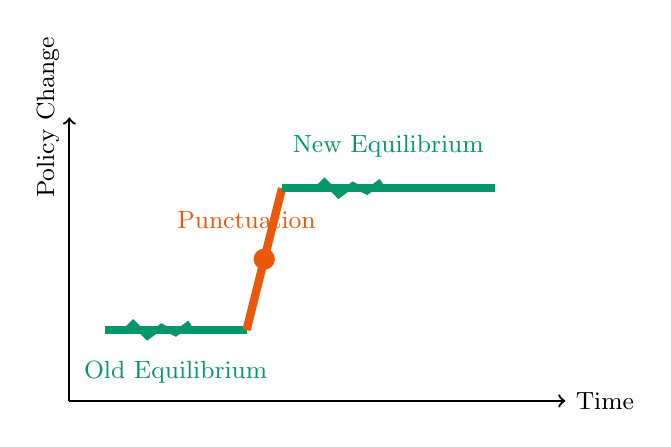
\begin{tikzpicture}[scale=0.9]
        % Axes
        \draw[->, thick] (0,0) -- (7,0) node[right] {\small Time};
        \draw[->, thick] (0,0) -- (0,4) node[above, rotate=90] {\small Policy Change};

        % Policy line with punctuation
        \draw[thick, equilibriumgreen, line width=3pt] (0.5,1) -- (2.5,1);
        \draw[thick, punctuationorange, line width=3pt] (2.5,1) -- (3,3);
        \draw[thick, equilibriumgreen, line width=3pt] (3,3) -- (6,3);

        % Mark the punctuation point
        \fill[punctuationorange] (2.75,2) circle (0.15);

        % Labels
        \node[below, text=equilibriumgreen, font=\small] at (1.5,0.7) {Old Equilibrium};
        \node[above, text=punctuationorange, font=\small] at (2.5,2.3) {Punctuation};
        \node[above, text=equilibriumgreen, font=\small] at (4.5,3.3) {New Equilibrium};

        % Add some minor fluctuations to show "normal" variation
        \draw[equilibriumgreen, line width=2pt] (0.8,1) -- (0.9,1.1) -- (1.1,0.9) -- (1.3,1.05) -- (1.5,0.95) -- (1.7,1.1);
        \draw[equilibriumgreen, line width=2pt] (3.5,3) -- (3.6,3.1) -- (3.8,2.9) -- (4.0,3.05) -- (4.2,2.95) -- (4.4,3.1);
      \end{tikzpicture}
    \end{center}
  \end{column}

  \begin{column}{0.45\textwidth}
    \begin{block}{Key Concepts}
      \pause
      \begin{itemize}
        \item \textbf{Policy Images}: How issues are understood and framed
        \item \textbf{Venue Shopping}: Moving issues to favorable decision-making venues
        \item \textbf{Attention Shifts}: Rapid changes in focus after long periods of inattention
      \end{itemize}
    \end{block}
  \end{column}
\end{columns}

\pause
\vspace{0.5cm}

\begin{alertblock}{Real-World Example:}
  Major civil rights legislation in the 1960s, which marked a sudden shift after years of incremental or no change, establishing a new policy equilibrium.
\end{alertblock}

\end{frame}

% Comparing Theories
\begin{frame}
\frametitle{Comparing the Theories}

\begin{table}
\centering
\small
\begin{tabular}{|p{2.3cm}|p{2.3cm}|p{2.5cm}|p{3cm}|}
\hline
\centering\textbf{Theory} & \centering\textbf{Focus} & \centering\textbf{Change Mechanism} & \centering\textbf{Key Insight} \\
\hline
\pause
\centering\textbf{Multiple Streams} & \centering Timing and opportunity & \centering Convergence of streams & \centering Windows of opportunity are rare and brief \\
\hline
\pause
\centering\textbf{Advocacy Coalition} & \centering Group dynamics & \centering Coalition competition & \centering Beliefs drive policy positions \\
\hline
\pause
\centering\textbf{Punctuated Equilibrium} & \centering Patterns over time & \centering Rapid shifts after stability & \centering Change is often episodic rather than gradual \\
\hline
\end{tabular}
\end{table}

\pause
\vspace{0.5cm}
\centering
Each theory provides valuable insights for different aspects of policy change

\end{frame}

% Application Case Study
\begin{frame}
\frametitle{Applying Theory to Policy Analysis}
\framesubtitle{Case Study: Healthcare Reform}

\begin{columns}
  \begin{column}{0.32\textwidth}
    \begin{block}{\textcolor{streamblue}{Multiple Streams}}
      \begin{itemize}
        \item \textbf{Problem}: Rising costs
        \item \textbf{Policy}: Different reform models
        \item \textbf{Politics}: Party control of government
      \end{itemize}
    \end{block}
  \end{column}

  \begin{column}{0.32\textwidth}
    \begin{block}{\textcolor{coalitionred}{Advocacy Coalition}}
      \begin{itemize}
        \item Progressive reform coalition
        \item Market-based reform coalition
        \item Status quo coalition
      \end{itemize}
    \end{block}
  \end{column}

  \begin{column}{0.32\textwidth}
    \begin{block}{\textcolor{punctuationorange}{Punctuated Equilibrium}}
      \begin{itemize}
        \item Long periods of debate
        \item Sudden passage of legislation
        \item New implementation equilibrium
      \end{itemize}
    \end{block}
  \end{column}
\end{columns}

\vspace{1cm}
\centering
Different theories highlight different aspects of the same policy story

\end{frame}

% Summary
\begin{frame}
\frametitle{Summary}

\begin{block}{Key Takeaways}
  \begin{itemize}
    \item Policy process theories help us understand and predict policy changes
    \item \textbf{Kingdon's Multiple Streams Framework} highlights the convergence of problem, policy, and politics streams
    \item The \textbf{Advocacy Coalition Framework} focuses on belief systems and coalition dynamics
    \item \textbf{Punctuated Equilibrium Theory} explains long periods of stability interrupted by sudden changes
  \end{itemize}
\end{block}

\vspace{1cm}

\begin{center}
  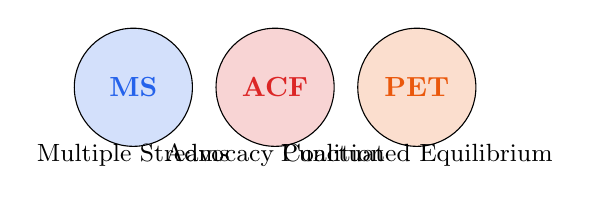
\begin{tikzpicture}[scale=0.6]
    % Create a visual summary with all three theory symbols
    \node[draw, circle, fill=streamblue!20, minimum size=1.5cm] at (0,0) {\textcolor{streamblue}{\textbf{MS}}};
    \node[draw, circle, fill=coalitionred!20, minimum size=1.5cm] at (3,0) {\textcolor{coalitionred}{\textbf{ACF}}};
    \node[draw, circle, fill=punctuationorange!20, minimum size=1.5cm] at (6,0) {\textcolor{punctuationorange}{\textbf{PET}}};

    \node[below] at (0,-1) {\small Multiple Streams};
    \node[below] at (3,-1) {\small Advocacy Coalition};
    \node[below] at (6,-1) {\small Punctuated Equilibrium};
  \end{tikzpicture}
\end{center}

\end{frame}

\end{document}
